\begin{flushleft}
\section*{Versuche}






\subsection*{Laboreinrichtung}


hier Foto von Versuchsaufbau allgemein, mit den drei Maschinen

\subsubsection*{Maschinensatz}








\begin{tabular}{|L{5cm}|l|c|c|c|c|}
 \hline
 \rowcolor[gray]{.8} \textbf{$Bez.$} & \textbf{$P_{Nenn}$} & \textbf{$p$} & \textbf{$f$} & \textbf{$Spannung$ $\Delta$ / $Y$} & \textbf{$n_{Nenn}$}  \\
 \hline
Synchronmaschine&8.7 kW &2 &50 Hz&220/380 V&1500 $\frac{1}{min}$\\
\hline
Gleichstrommaschine&8.5 kW & - & - & 220 VDC& 1500 $\frac{1}{min}$\\
\hline
Schleifring ASM &10 kW &2&50 Hz& 230/400 V& 1420 $\frac{1}{min}$\\
\hline

\end{tabular}






\subsubsection*{Messeinrichtungen}




\begin{tabular}{|L{0.8 \textwidth}|l|}
 \hline
 \rowcolor[gray]{.8} \textbf{Bezeichnung} & \textbf{Nr}  \\
 \hline
 Messtrennverstärker 1  & xxx  \\
\hline
Messtrennverstärker 2  & xxx  \\
\hline
Amperezange  & xxx  \\
\hline
Oszilloskop  & xxx  \\
\hline
Multimeter  & xxx  \\
\hline
Drehzahl-und Drehmomentmessung  & -  \\
\hline
Polradwinkel-Messgerät  & -  \\
\hline
Dreiphasiges Leistungsmessgerät PM 3000  & -  \\
\hline
Wattmeter   & -  \\
\hline
\end{tabular}


\subsubsection*{Speisungen und Belastungen}

\begin{tabular}{|L{0.3 \textwidth}|l|}
 \hline
 \rowcolor[gray]{.8} \textbf{Bezeichnung} & \textbf{Anwendungszweck}  \\
 \hline
 Chopper  & zur Erregung der SM  \\
\hline
Kastenwiderstand & Belastung ohmsch  \\
\hline
 Variac Einrichtung & Belastung reaktiv  \\
\hline

\end{tabular}



\newpage
\subsection*{Inbetriebsetzung}
Als erstes sollen die Gleichstrommaschine sowie die ASM in Betrieb genommen werden und für die folgenden Messungen eingestellt werden.
\subsubsection*{Gleichstrommaschine}
Die GM wird so eingestellt, dass sie beim Einschalten auf eine Drehzahl von 1500 $\frac{1}{min}$ hochfährt. Dies entspricht gerade der Nenndrehzahl der SM.

\subsubsection*{ASM}
Die Asynchronmaschine wird im späteren Verlauf als Dämpfung für den SM genutzt. 
Da es sich um eine Schleifringläufer ASM handelt, kann über den Rotorkreis ein Widerstand zugeschalten werden. Dieser begrenzt den Anlaufstrom. Nach dem Hochfahren werden die Schleifringe kurzgeschlossen und die ASM kann als Kurzschlussläufer betrachtet werden.


\newpage



\subsection*{Maschinenkennwerte}
In diesem Abschnitt werden die charakteristischen Kennwerte der SM ermittelt.

\subsubsection*{Leerlaufkennlinie}
Mit der Leerlaufkennlinie wird der Zusammenhang der induzierten Phasenspannung (Effektivwert) in Abhängigkeit des Erregerstroms dargestellt. Für diesen Versuch muss die SM mit der Gleichstrommaschine bei Nenndrehzahl gehalten werden (1500 $\frac{1}{min}$).
Da die SM unbelastet ist, fliesst kein Strom $I_1$ durch die Statorwicklung, $\Delta U$ beträgt 0 und die Polradspannung (induzierte Spannung) entspricht der Phasenspannung $U_1$ resp. $U_{ph}$. \\


\begin{figure}[H]
    \centering
        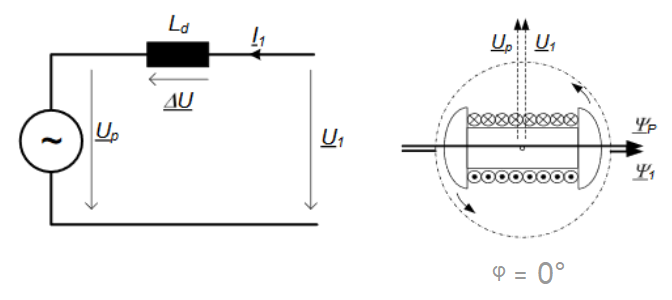
\includegraphics[ %trim=0.5cm 0.5cm 0.5cm 0.5cm,
         scale = 0.7]{leerlauf}
         \caption[]{Leerlaufbetrieb \footnotemark}
    \label{fig:abb1}
\end{figure}

\footnotetext{Aus dem Skript 'Leistungselektronik und elektrische Antriebe' Kapitel 'Drehfeldmaschinen'}




\begin{figure}[H]
    \centering
        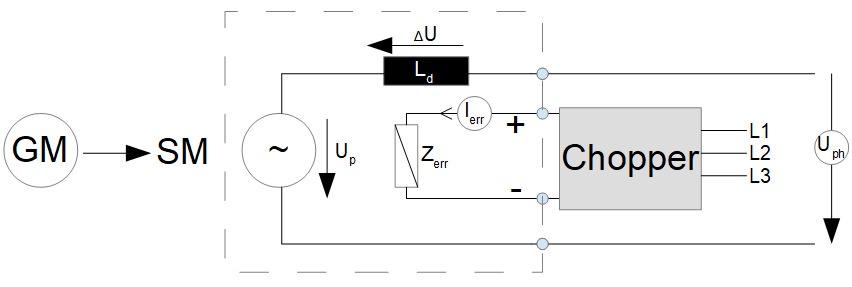
\includegraphics[ %trim=0.5cm 0.5cm 0.5cm 0.5cm,
         scale = 0.6]{leerlauf_schema}
    \caption{Schaltungsaufbau im VZS}
    \label{fig:abb1}
\end{figure}









\newpage



\begin{figure}[H]
    \centering
        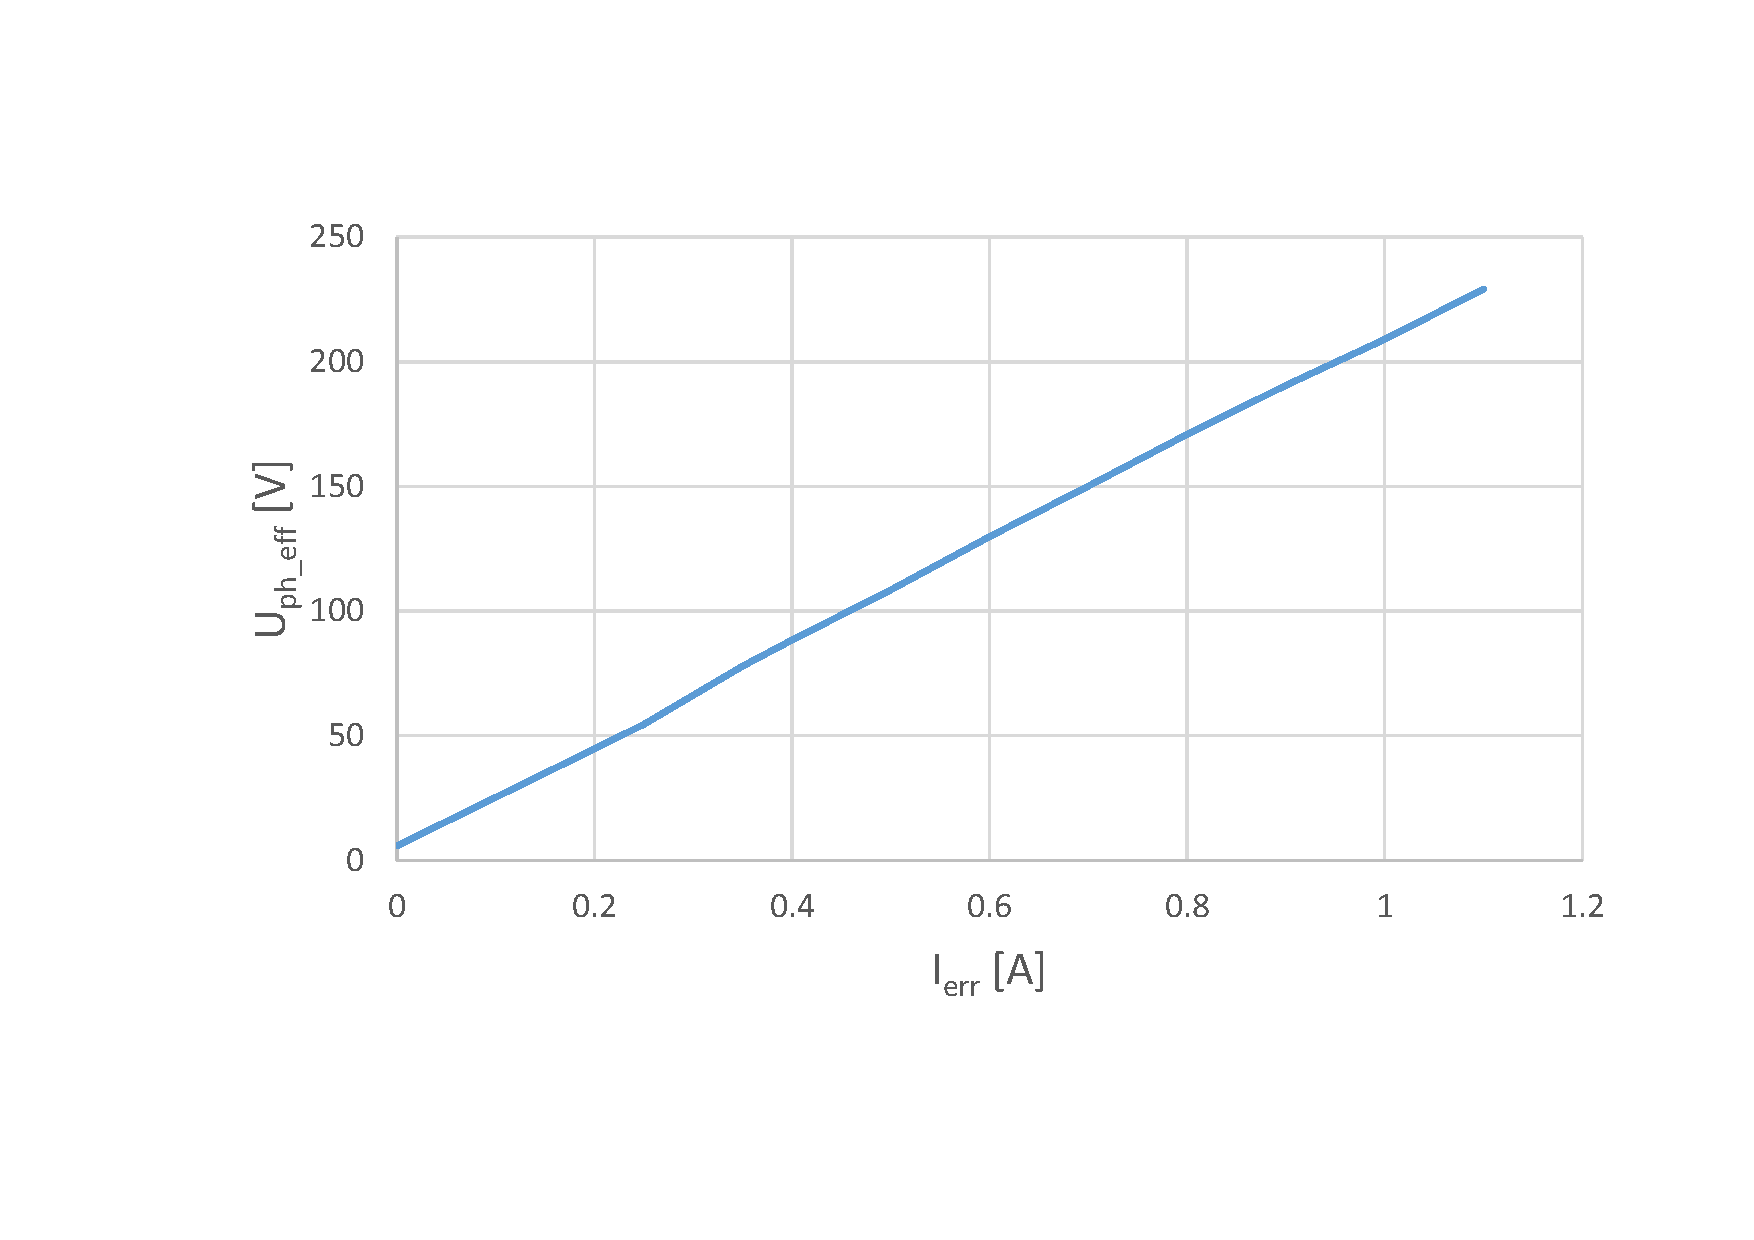
\includegraphics[ %trim=0.5cm 0.5cm 0.5cm 0.5cm,
         width=0.80\textwidth]{versuch_Uph_I_err.pdf}
    \caption{Phasenspannung in Abhängigkeit des Erregerstroms}
    \label{fig:abb1}
\end{figure}



Der Grafik ist zu entnehmen, dass die Phasenspannung durch das Erhöhen des Erregerstroms linear zunimmt. 
Die Kennlinie entspricht der Magnetisierungskennlinie der Synchronmaschine.\\


\vspace{0.4cm}
\textbf{Verwendete Messwerkzeuge}: Multimeter ($I_{err}$), Oszilloskop und\\ Messtrennverstärker 1($U_{ph}$)

\newpage






\subsubsection*{Kurzschlusskennlinie}

Im Kurzschlussfall($U_1$ = 0V) fällt die induzierte Spannung $U_p$ über der Statorwicklung $\Delta U$ ab. Abhängig vom Erregerstrom verändert sich die induzierte Spannung und somit auch der Phasenstrom $I_1$ resp. $I_{ph}$.
Mit der Kurzschlusskennlinie soll dieser Zusammenhang grafisch dargestellt werden.
Auch in diesem Aufbau wird die SM mit der Gleichstrommaschine bei der Nenndrehzahl   betrieben.
 
 
\begin{figure}[H]
    \centering
        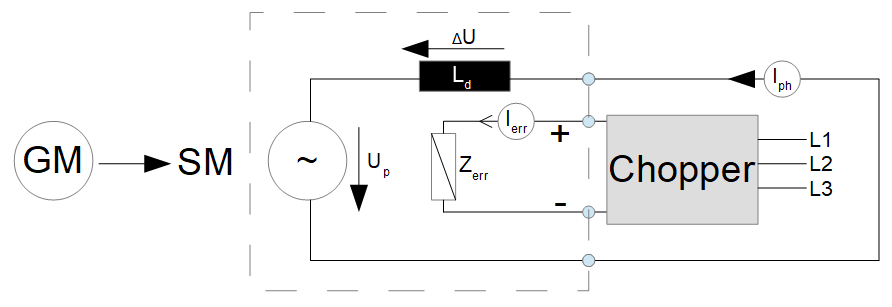
\includegraphics[ %trim=0.5cm 0.5cm 0.5cm 0.5cm,
         scale = 0.6]{kurzschluss_schema}
    \caption{Schaltungsaufbau im VZS}
    \label{fig:abb1}
\end{figure}



\begin{figure}[H]
    \centering
        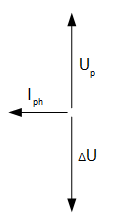
\includegraphics[ %trim=0.5cm 0.5cm 0.5cm 0.5cm,
         scale = 0.8]{zps_kurzschluss}
    \caption{Zeigferdiagramm im VZS}
    \label{fig:abb1}
\end{figure}


\begin{figure}[H]
    \centering
        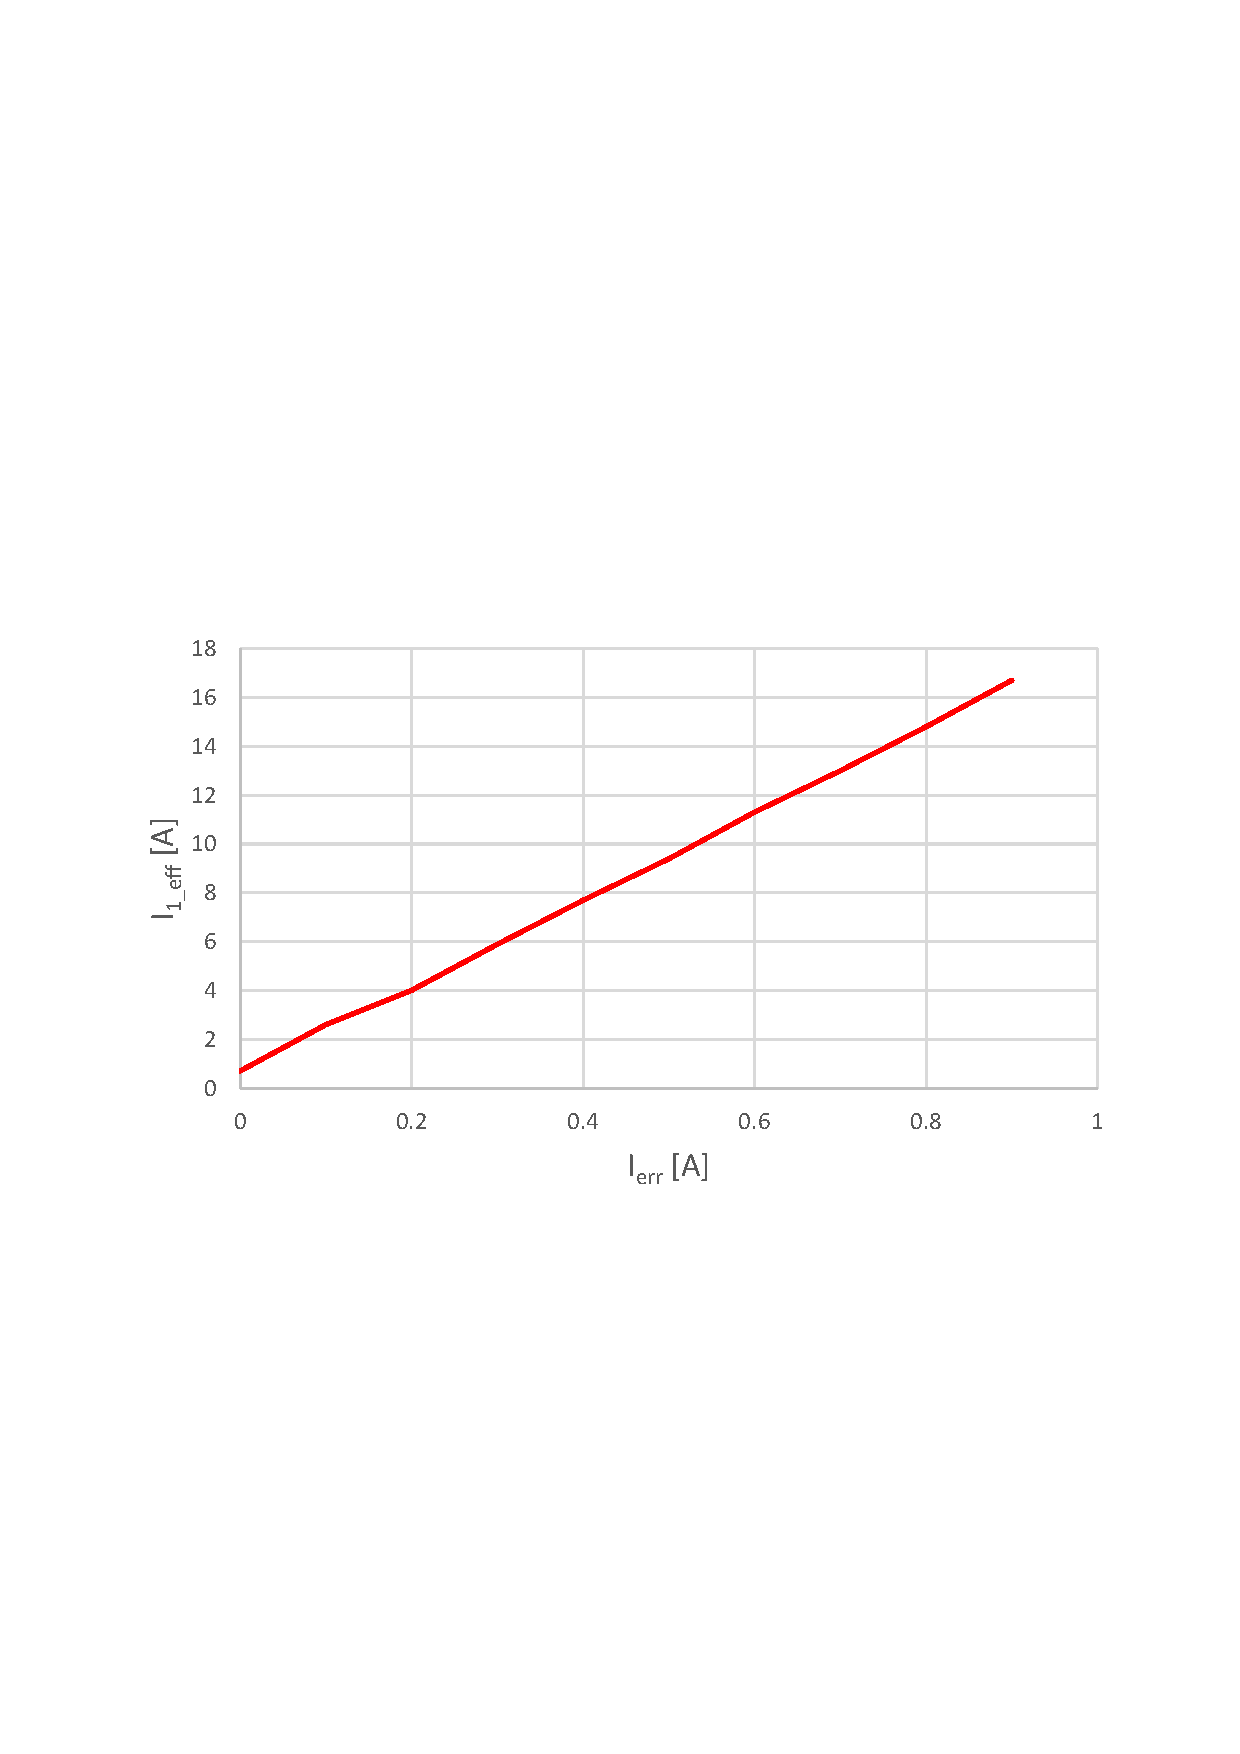
\includegraphics[ %trim=0.5cm 0.5cm 0.5cm 0.5cm,
         width=0.80\textwidth]{versuch_I_ph_I_err.pdf}
    \caption{Phasenstrom in Abhängigkeit des Erregerstroms}
    \label{fig:abb1}
\end{figure}

Auch die Kurzschlusskennlinie verhält sich linear. Der Effektivwert des Phasenstroms nimmt proportional zum Erregerstrom zu.\\

\vspace{0.4cm}
\textbf{Verwendete Messwerkzeuge}: Multimeter ($I_{err}$), Oszilloskop und Amperezange($I_{ph}$) 




\newpage
\subsubsection*{Längsreaktanz $X_d$}

Anhand der Messresultat vom Leerlauf-resp. Kurzschlussversuch lässt sich die Längsreaktanz $X_d$ berechnen. Da die SM mit der Nenndrehzahl betrieben wurde, dreht sich der Rotor mit der selben Winkelgeschwindigkeit wie das Statordrehfeld. In diesem Betriebsfall kann entsprechend nur die Längsreaktanz bestimmt werden.\\

Es gilt:\\

\vspace{0.3cm}
$$\underline{\Delta U} = j \cdot X_d \cdot \underline{I_1}$$
resp:\\
\vspace{0.3cm}
$$ X_d = \frac{\underline{\Delta U}}{j \cdot \underline{I_1}}  = 2 \cdot \pi \cdot f \cdot L_d$$\\

\vspace{0.5cm}


Im Leerlauffall gilt unter Vernachlässigung des Wicklungswiderstands vom Stator \\$\Delta U$ = $\underline{U_{1}}$. \\
Der Phasenstrom $I_1$ kann, bei selbem Erregerstrom, der Kennlinie beim Kurzschlussversuch entnommen werden. Für einen Erregerstrom von 0.4A ergibt sich:\\
\vspace{0.3cm}
\begin{itemize}
\item $\underline{U_{ph_eff}} = \Delta U = $ 150 V
\item $\underline{I_{1_eff}} = $ 8 A
\end{itemize}


und somit:

$$\underline{\underline{L_d}} = \frac{150 V }{j \cdot 8 A \cdot 2 \cdot \pi \cdot 50 Hz} = \underline{\underline{59.7 mH}}$$





\end{flushleft}